%Latex Header

\documentclass[letterpaper]{report}

\usepackage{geometry}
\geometry{letterpaper, landscape, margin=1.5in}
\usepackage{multicol}
\usepackage{verbatim}

\usepackage{fontspec}
\usepackage{amsmath}
%\usepackage[MnSymbol]{mathspec}
\usepackage{mathpazo}
\setmainfont
     [ BoldFont       = texgyrepagella-bold.otf ,
       ItalicFont     = texgyrepagella-italic.otf ,
       BoldItalicFont = texgyrepagella-bolditalic.otf ]
     {texgyrepagella-regular.otf}
\setmainfont{Gill Sans MT}

\usepackage[english]{babel}
\usepackage[utf8]{inputenc}
\usepackage{graphicx}
\usepackage[colorinlistoftodos]{todonotes}
\usepackage{physics}

\usepackage{lipsum}

\renewcommand{\thesection}{\arabic{section}}
\renewcommand{\thesubsection}{\thesection.\alph{subsection}}
\renewcommand{\thesubsubsection}{(\roman{subsubsection})}

\title{Collaborative, Contact-Based Schemas for Robot Righting utilizing Hull Shape Design}
%Collaborative Collision- and Contact-based Schemes for Robot Roll Righting (c3r3)

\author{David McPherson}

\date{Autumn 2017}

\begin{document}

\maketitle
\global\csname @topnum\endcsname 0
\global\csname @botnum\endcsname 0

\begin{abstract}
Two are better than one. This truism is the foundation and the motive force that birthed society.
Naturally, we want to imbue this power into our metal children.
Imitating birds and fish, we built swarms that could keep formation via elegant decentralized control algorithms.
Inspired by ants, we applied formation keeping to carrying loads as a mobile robot team.
In this work, we further specialize this collaborative manipulation to moving other team mates thereby creating collaborative locomotion.
Our design space is enriched by designing both the manipulator and the manipulatee at the same time.
Traditional collaborative manipulation work focuses on manipulating objects in the same plane of movement as the mobile robots and adheres strictly to form or force closure manipulation paradigms.
Our new design richness allows us to leverage work on in-hand, dexterous manipulation and dynamic manipulation techniques to manipulate objects (now teammates) in degrees of freedom (DOF) outside our plane of movement.
These further manipulation DOF are accessed by especial care in designing the contact surfaces between robots which allows us to guide objects while slipping, instead of rigidly demanding complete closure.
This paper will demonstrate the collaborative locomotion concept in the simplest possible cooperative maneuver: rolling a pronated robot back onto its feet (adding a previously inaccessible roll DOF to a differentially driven robot).
Within this showcase application we discover several possible designs for cooperative righting strategies.
The strategies follow the traditional manipulation classification framework: kinematic, quasi-static, and dynamic.
We investigate each method analytically as well as implementing the best method on real robots.

\begin{figure}[h]
\centering
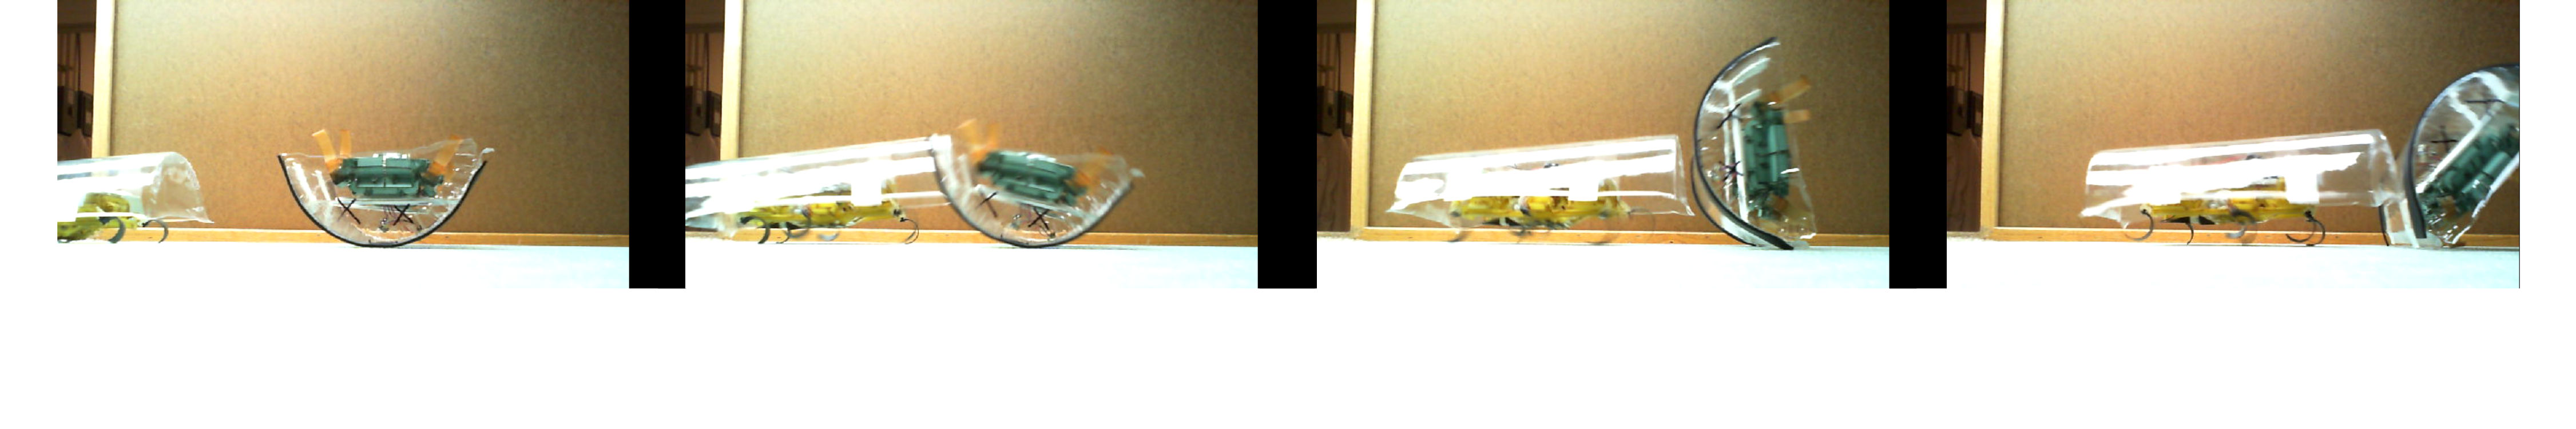
\includegraphics[width=1.0\textwidth]{KinFlipStrip3.png}
%\caption{Frame sequence of RoACH team performing our cooperative righting maneuver on styrofoam}
\end{figure}
\end{abstract}

\section{Introduction}
Humanity's greatest strength is our social prowess; clearly we want to bestow this greatest of all gifts to our silicon offspring.
Even animals exhibit social behavior that result in some of the most awe-inspring feats in the animal kingdom.
Dolphins leaping in unison, birds soaring in tight formation, and ants carrying away feasts spark the imagination of children and engineers alike.
It should come as no suprise, then, that roboticists have striven for decades to imbue robots with that selfsame social spark.
And we have succeeded to some extent.
Decentralized control strategies inspired by flying birds \cite{reynolds1987flocks} produce tight formation controls for our flying robots \cite{RealBoids}.
This newfound capacity for formation control enabled cooperative manipulation of objects \cite{rus1995moving,sugar2002control,spletzer2001cooperative,song2002potential} just like ants \cite{kube2000cooperative}.
We take this a step further by having teams manipulate a very special object: another team member.
With the team's help a robot can gain new ways of moving.
Our goal moves from cooperative manipulation to cooperative locomotion.
The design freedom granted by specializing manipulation to other teammates allows us to create more rich manipulations than mere translations.
By leveraging work in dynamic manipulation, we can design mobile robots that can rotate each other out of the plane of movement.

\subsection{Structure of Thesis}
This Thesis first exposits the rich tradition of research this work builds upon in Section 1.
We then detail the hardware used in our experiments in Section 2 for the sake of reproducibility.
The next three sections each investigate a different schema for cooperative righting.
We follow the manipulation taxonomy expounded upon in Mason's seminal text ``Mechanics of Robotic Manipulation'' \cite{MasonMORMBook}: Kinematic, Static\footnote{Interestingly, static righting corresponds to passive self-righting by placing the center of gravity above the center of rotation. Static righting is non-cooperative and so doesn't receive a treatment here (static manipulation also did not receive its own chapter in ``Mechanics of Robotic Manipulation'' \cite{MasonMORMBook})}, Quasi-static, Dynamic.
Section 3 investigates a two robot (coresponding to a ``two-finger'' manipulation) maneuver that rolls a pronated third robot back onto its feet.
The two robots fully constrain the third robot and closing the distance between the two kinematically moves the third through a full roll re-orientation.
This method is purely kinematic.

\begin{figure}[h]
\centering
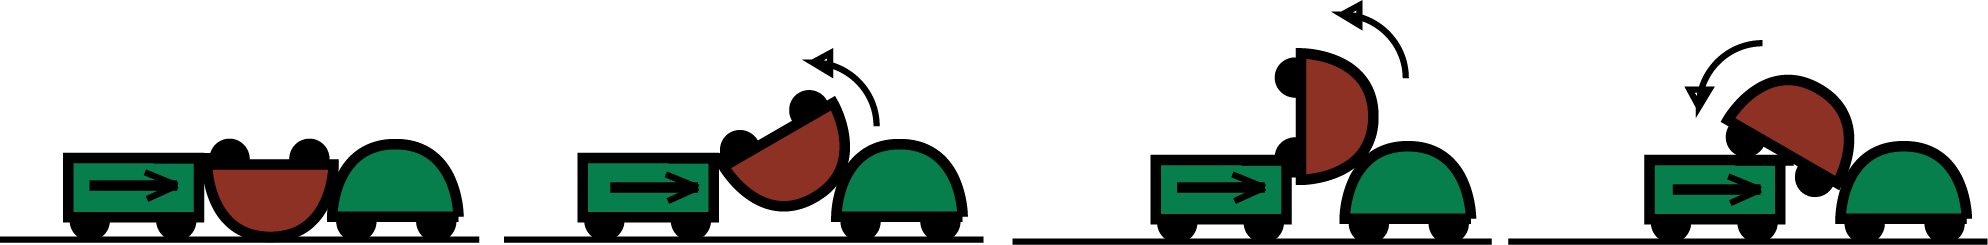
\includegraphics[width=1.0\textwidth]{Kinematic_CoopCartoon.png}
\caption{Cartoon of ``Kinematic'' Cooperative Flip Technique}
\end{figure}

Section 4 moves to a single robot locomoting the pronated robot. With the loss of fully constrained control, the cooperative locomotion method must compensate by leveraging previously unmodeled effects.
Previously neglected ground friction forces now become our ally providing the necessary second force to create a moment couple on the pronated robot.
In this sense the ground could be interpreted as a second finger, but is more proximal to the palm in human dexterous manipulation.
By introducing frictional forces we leave the domain of kinematic manipulation and enter quasi-static analysis, making this the quasi-static flipping method.

\begin{figure}[h]
\centering
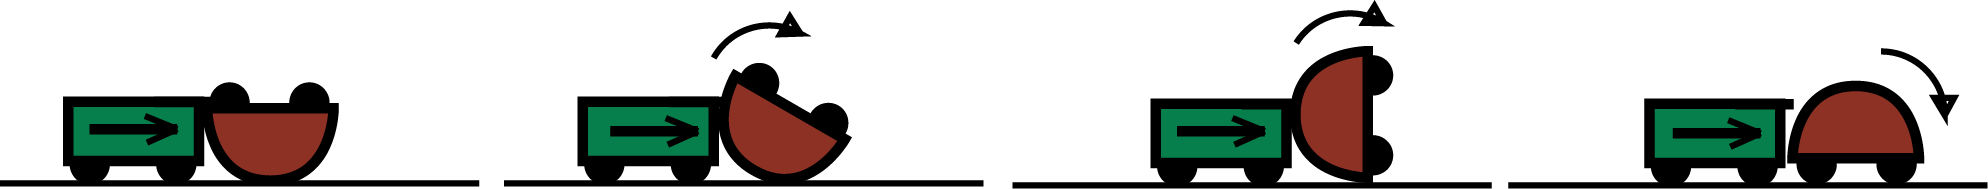
\includegraphics[width=1.0\textwidth]{QuasiStatic_CoopCartoon.png}
\caption{Cartoon of ``Quasi-static'' Cooperative Flip Technique}
\end{figure}

We will see that this enabling insight will also become the quasi-static flip's major short-coming: sensitivity to ground-shell friction coefficients.
The final flipping method eschews this constraint by relying on the inertial pseudo-force to couple with a ballistic push from the compatriot robot to create the moment couple.

\begin{figure}[h]
\centering
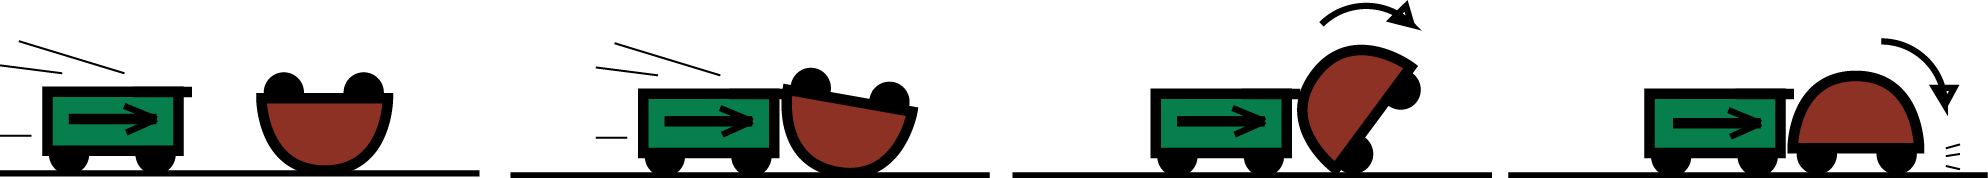
\includegraphics[width=1.0\textwidth]{Dynamic_CoopCartoon.png}
\caption{Cartoon of ``Dynamic'' Cooperative Flip Technique}
\end{figure}

\section{Related Work}

This work is strongly rooted in the grasping and automated manipulation literary tradition.
It weds three separate branches of this rich field to investigate a new class of behaviors and manipulations.
We weave together work on cage-free manipulation, team manipulation, and self manipulation.

\subsection{Team Manipulation}
Classic grasping work focuses on placing multiple fingers to yield form closure or force closure by keeping all disturbances and wrenches within the friction cone.
Team manipulation ports these concepts by simply viewing each robot as a separate finger and using a team of mobile robots to grasp and manipulate an object.
This idea was spearheaded and popularized by Daniela Rus in her seminal work on furniture moving robots \cite{rus1995moving}.
The idea was evolved and matured by Vijay Kumar's group to include tactile feedback \cite{sugar2002control}, vision-based formation keeping \cite{spletzer2001cooperative}, and elegant decentralized control methods \cite{song2002potential}.
However, these works can only achieve manipulation within the plane that the mobile robots drive upon.
I am interested in adding out of plane rolling capabilty to a mobile team manipulator.

\subsection{Cage-Free Manipulation}
I accomplish this feat by tapping into cage-free manipulation techniques that embrace dynamics and askew forces to create more complex manipulations.
Beautiful examples of this elegant manipulation philosophy is championed by Matt Mason's Manipulation Lab \cite{lynch1999dynamic}\cite{dafle2014extrinsic}.
My work particularly pulls upon his student Alex Rodriguez's work on shape design that molds the normal forces applied throughout a surface contact interaction to achieve the desired manipulation \cite{rodriguez2013effector}.

\subsection{Cooperative Locomotion}
Rather than manipulate arbitrary objects we investigate the exciting case of cooperative locomotion: where the manipulated object is another robot teammate.
This structure simplifies the problem by allowing us to co-design both the manipulator and the manipulatee for optimal manipulability.
To our knowledge, a manipulation-based approach to cooperative locomotion is novel.

The closest comparison are other cooperative locomotion projects such as the cooperative step climbing work by Casarez \cite{casarez2016step} where teammates boost each other via a magnetic hinge connection and pull each other up via a tether.
Biomimetic approaches such as the TERMES \cite{werfel2014designing} construction team that could collaborataively build bridges, steps, or other locomotive affordances.

\subsection{Self Righting}
In this work we focus on the cooperative locomotion example of cooperative righting.
Therefore, we should compare this work to alternative righting schemes that utilize an individual robot's spare degrees of freedom to effect a roll.
For example, Li et al. \cite{li2016cockroach} added special purpose biomimetic mechanisms for self-righting inspired by beetles' wings.
Similarly, Casarez and Fearing \cite{casarezTailRighting} demonstrate how adding an extra motorized tail can provide a self-righting behavior.
Saranli et al. \cite{saranli2004model} use the actuators they already have to roll: by flailing the robot's legs they can induce a roll moment on the body.

\subsubsection{Rightability}
Turtle \cite{domokos2008geometry}
Kessens \cite{kessens2012framework,kessens2014metric}

\section{Hardware}

\subsection{Robotic Platform}
The VelociRoACH is a Robotic Autonomous Crawling Hexapod (RoACH) experimental platform designed for high velocity running through its elegant minimal hardware design \cite{haldaneVelociRoACHDesign}.
This design makes the VelociRoACH a fertile showcase for dynamic maneuvers; it has broken speed records before \cite{haldane2015running}.
Due to its low cost and rapid manufacturing process, teams of RoACHes are a pragmatic platform for investigating multi-robot maneuvers \cite{casarez2016step}.
We will leverage these two boons to demonstrate dynamic, multi-robot maneuvers.

% Picture of VelociRoACH here.

We accomplish our cooperative locomotion through dynamic and dexterous manipulation techniques.
These techniques rely upon molding the force vectors that are applied throughout by the manipulation contacts.
These contact forces are governed by the shape and material of the outer hull of the robot.
By adding shells to our robotic platform we can mold the reaction force landscape to suit our purposes.
This was used in Li \cite{ChenTerradynamic} to affect how environmental obstacles push on the robot while traversing cluttered terrain.
Whereas Li sought to use reaction forces to disengage from objects, we instead employ these forces to manipulate said objects.
Therefore, the crux of our work is designing the shell shapes for our robot.

\begin{table}[tb]
% increase table row spacing, adjust to taste
\renewcommand{\arraystretch}{1.1}
\caption{Physical Parameters of VelociRoACH and Shell}
%\vspace{-0.1in}
\label{tab:Dimensions1}
\centering
\begin{tabular}{l c c}
\hline
Parameter name & Symbol & Value \\
\hline
Body mass & $m_b$ & $54.1$ g \\
Overall width, depth, height & $(w, h)$ & $(10, 19, 10)$ cm \\
Shell circular radius & $r$ & $5.0$ cm \\
Shell major, minor axis radius & $(r, b)$ & $(5.0, 3.5)$ cm \\
Shell center offset height & $d_{circle}$ & $11.4$ mm \\
                           & $d_{ellipse}$ & $7.27$ mm \\
Shell-shell contact friction coefficient & $\mu$ & $0.52$ \\
Shell-ground contact friction coefficient & $h$ & $0.26$ \\
...with rubberized strips on shell  & $h_{rubberized}$ & $1.07$ \\
\hline
\end{tabular}
\end{table}

\subsection{Shell Construction}
Shell shapes are the central design problem. Therefore, the design cycle of the shell is of utmost import.
To expedite the rate of design iterations, I refined the shell manufacture process by removing the primary bottleneck: speeding mold creation from days to hours.
\subsubsection{Mold Prototyping}
\label{sec:Molds}
Previously, in our lab we used additive manufacturing to print a mold for the shell shape.
This required multi-day printing sessions to manufacture a piece measuring 10x19x10 centimetres.
The printed thermoplastic mold would then be coated with paint so that it could withstand the molten plastic it was designed to mold in the vacuum former.
Although this method allowed nigh-infinite design freedom for shell shape, it was unacceptably slow and costly for the rate at which I needed to produce shells.
The solution I have pioneered sacrifices design flexibility for prototyping rapidity.

Our analysis will planarize the three-dimensional problem as we focus on actuating the roll degree of freedom.
Therefore, we are only interested in the two-dimensional profile of the shell and should eliminate secondary curvature along the depth-axis to prevent unwanted yaw rotations and other confounding effects.
This deisgn goal implies that all shell designs should be prisms.
A prism's hull can be created with a single continuous sheet folded over the two-dimensional profile which defines the type of prism (e.g. rectangular prism, cylinder, elliptical prism, extruded polygon, etc.).
Constructing prismatic shells via single-sheet folding replaces the bottleneck of additive-manufacturing.

A contoured single sheet of cardstock will crumple under the vacuum pressure in a vacuum former.
We must add a supporting skeleton to brace the cardstock.
The skeleton must support pressure that points uniformly along the normals of the surface.
Since it is exerted normally, a mere square honeycomb is insufficient.
Instead, supporting beams directed along the normal must be used in the style of a Viking longhouse.
A traditional rectilinear honeycomb can then be used to supplement and hold the beams in place.
A picture of the supporting skeleton is shown in Fig. \ref{fig:ManufactureSkeleton}

\begin{figure}[ht]
\centering
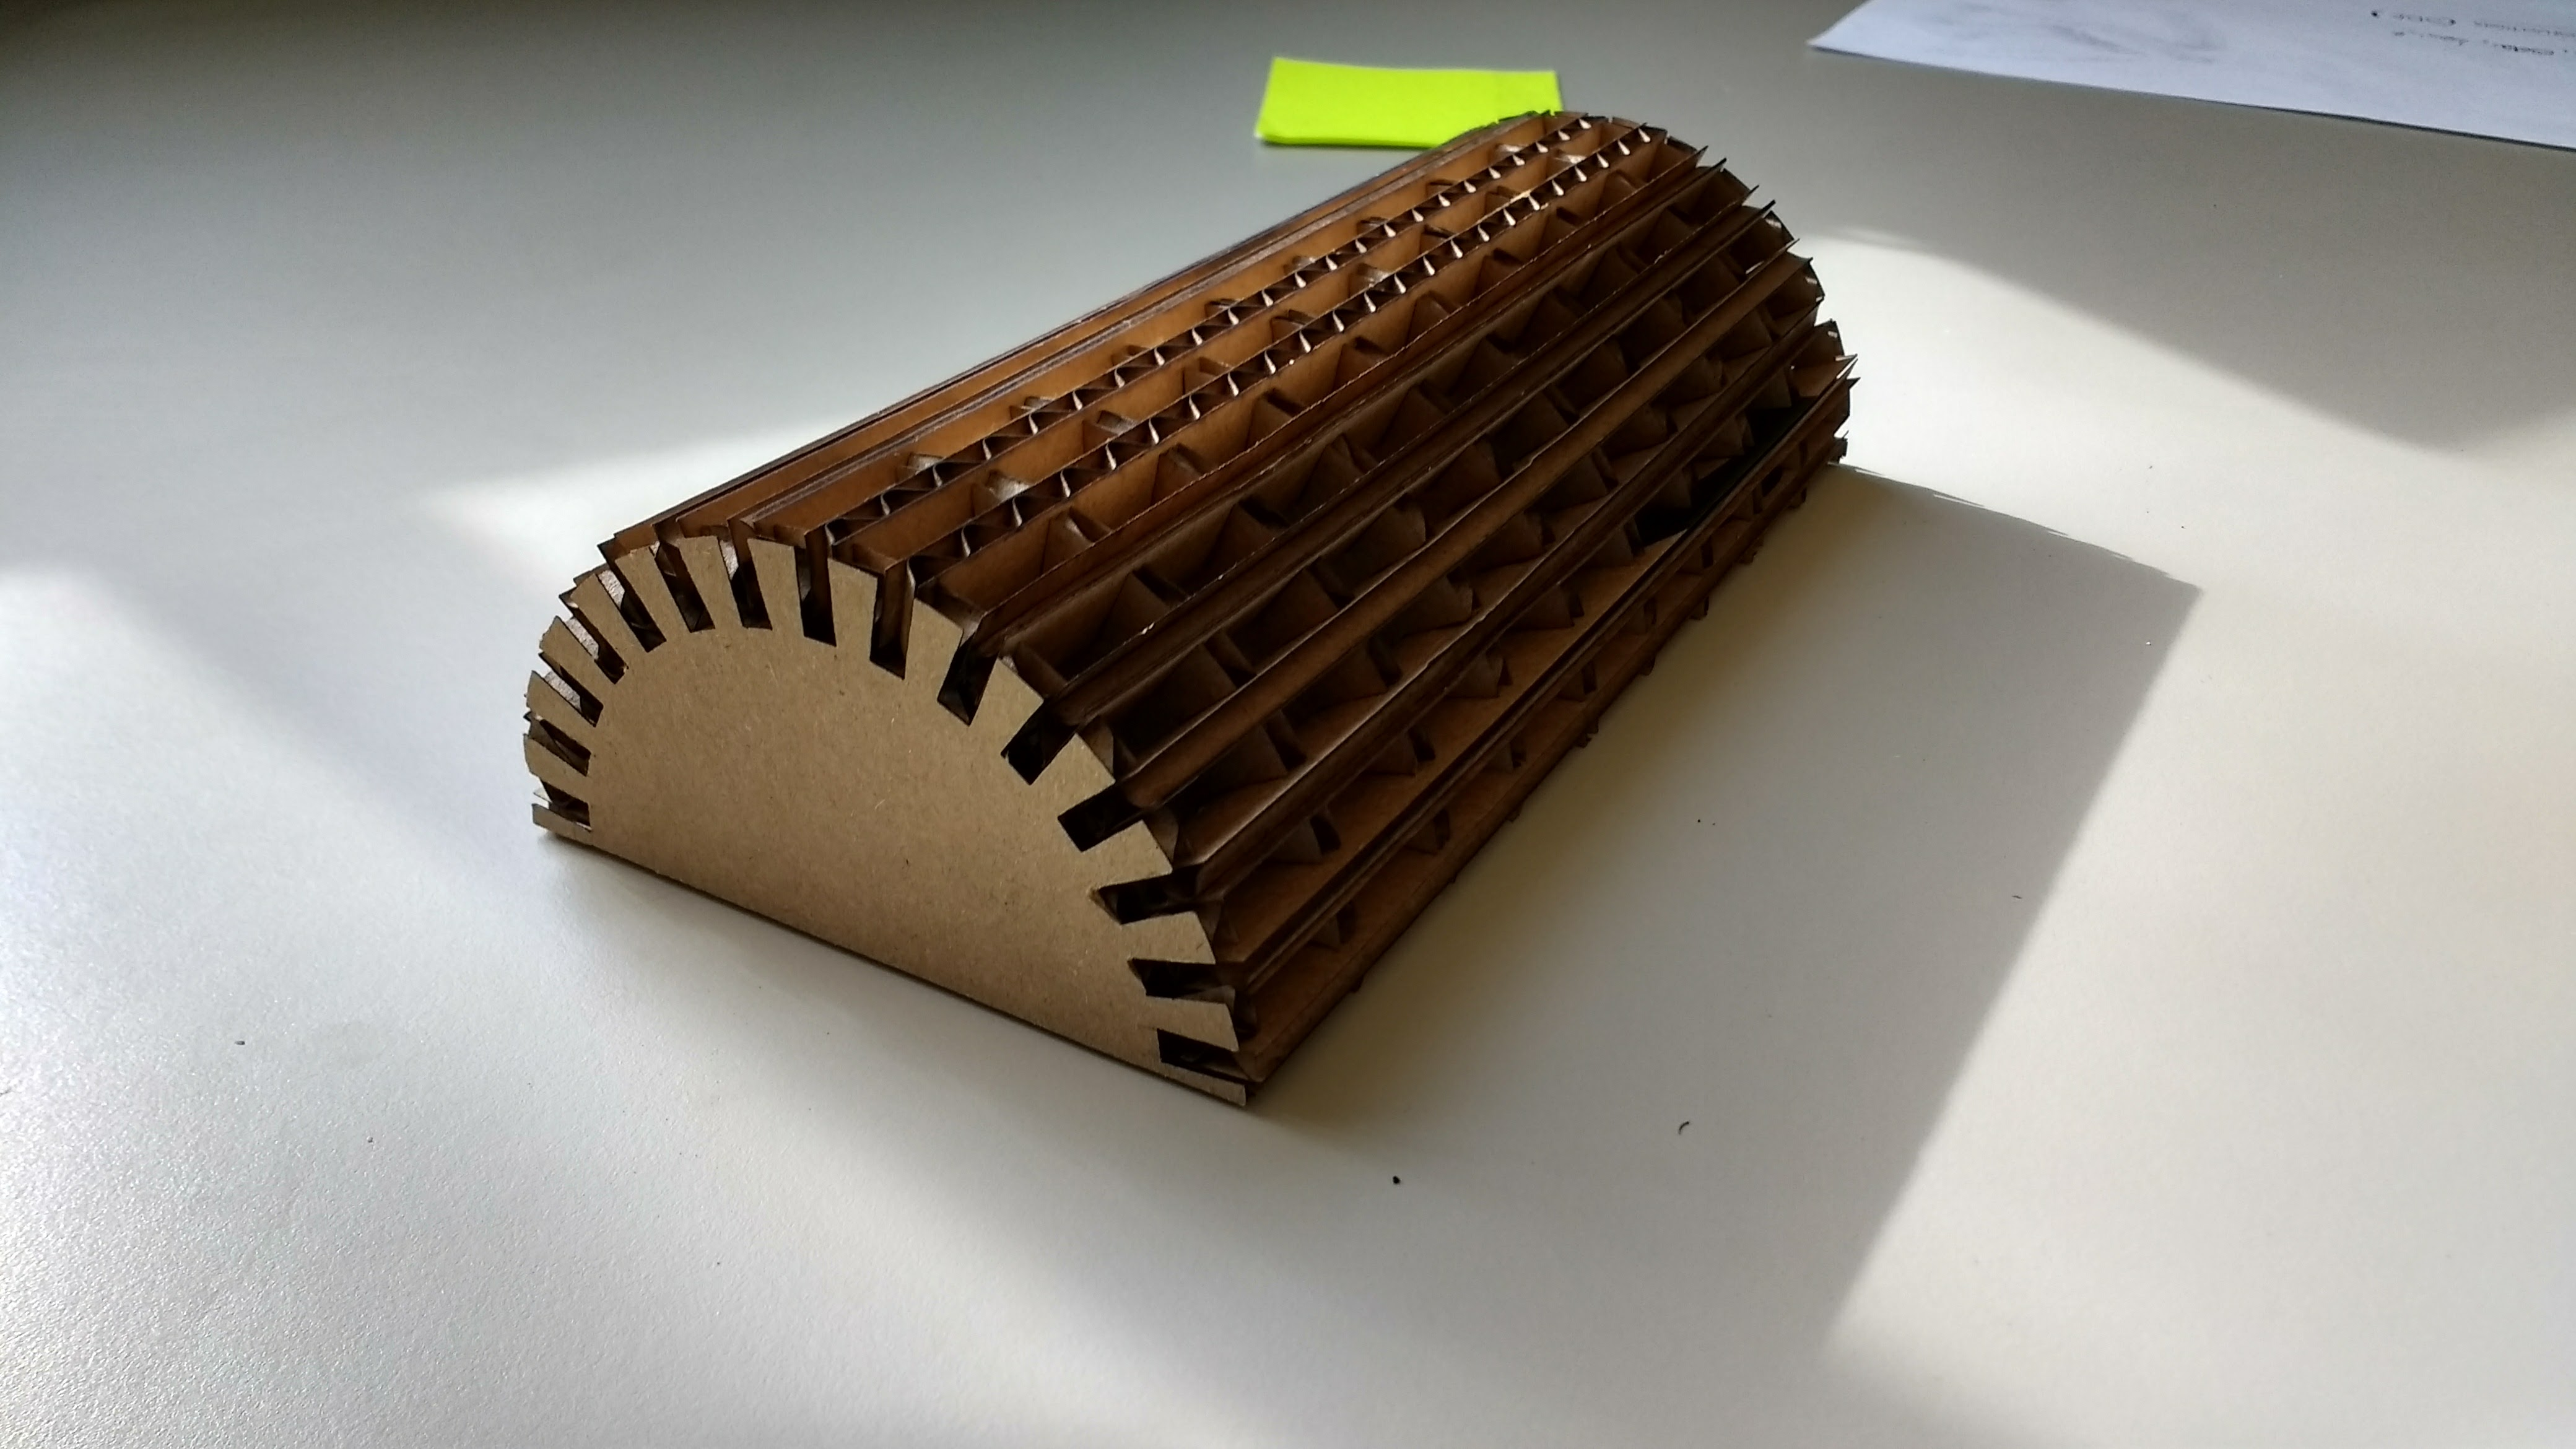
\includegraphics[width=0.4\textwidth]{SupportingSkeleton.jpg}
\caption{\label{fig:ManufactureSkeleton}Supporting Skeleton fully Assembled}
\end{figure}

The cardstock can now be wrapped tightly around the supporting skeleton.
To enable tight cinching and hands free fixturing, a rectangular jig with a cutout in the shape of the mold footprint is used.
The skeleton is then held in place whilst the cardstock is slipped between the skeleton and the jig.
The cardstock is pulled taut (so as to avoid wrinkles forming during the suction event) and glued to the skeleton.
The completed mold is now ready to be used in the vacuum former to shape plastic shells.

\subsubsection{Standard Magnet Mount}
Once the plastic shells are formed to the desired prismatic shape, they are mounted to the robot via modular magnetic mounts.
A cardstock strip is cut to length according to the formula:

$$
l_{mountstrip} = 2 \sqrt{r^2 - h_m^2} + 2 (\sin^{-1}(h_m/r) r)
$$

where $h_m$ is the height in the shell you want to mount the robot.
For our experiments we choose $h_m = r/2 = 25$ mm resulting in:

$$
l_{mountstrip} = 2 (\sqrt{3} \frac{r}{2}) + 2 (\frac{\pi}{6} r) = (\sqrt{3} + \frac{\pi}{3} ) r
$$

We chose $h_m = 25$mm which mandated that $l_{mountstrip} = 139$ mm.
The strip was then affixed to the shell via permanent adhesive. The adhesive used was LOCTITE495 Instant Adhesive.

\section{Kinematic Flip Method}

\begin{comment}
\subsection{Design Evolution}
The design started by exclusively examining the design of the pushing robot's contact surface, oblivious of the design choices inherent in the shape of the robot we were pushing (which was the ellipsoidal shape already extant in our lab from \cite{ChenTerradynamic}) and choice of backstop to push against (which we assumed was a suitable, external, environment fixture).
We started by shaping the plow as the inverse of the turtled robots' ellipsoidal shape.
This curved front plow resembled a snow shovel.
However, we quickly realized that the robot only contacted one slope on this curved surface throughout the pushing procedure, allowing us to simplify the spline into fewer and fewer approximating lines until it was a just a single sloped surface.
Inspired by robust grasping research, we also experimented with a cylindrical pushing surface, which worked fantastically.
This was the point where my research hit a road block from discouragement about the apparent triviality of designing a plow for righting (apparently any shape I could try would work)!

I realized that the power in this design was actually in the co-design of manipulator and manipulatee and that I had blindly initialized to an extremely good turtled robot shell.
I also realized that my assumptions about having a backstop fixture could be made more practical by instituting a third robot as a backstop robot.
Upon this realization I made the backstop the cylindrical surface and made the wall become a moving robot instead.
This streamlined the number of specialized manipulation surfaces needed.
\end{comment}

\subsection{Kinematic Analysis}
This flipping method is termed the ``Kinematic Flip'' since the flipping action is due purely to contact constraints that geometrically force the pronated robot through a series of poses up to the tipping point.

\begin{figure}[ht]
\centering
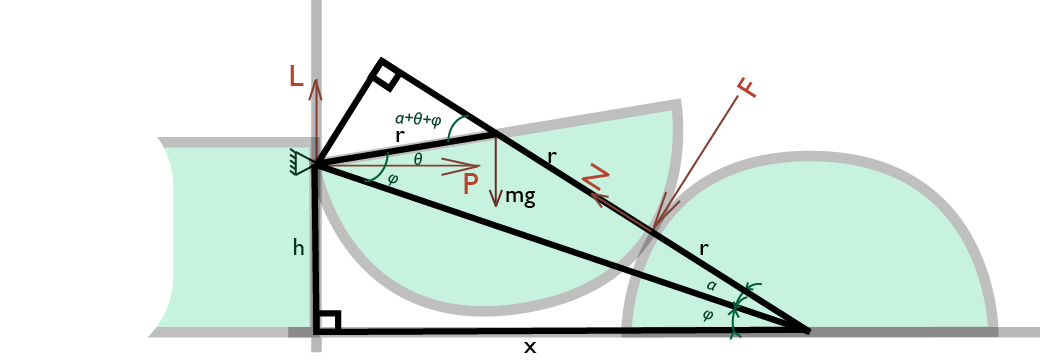
\includegraphics[width=0.5\textwidth]{Kin_FreeBodyDiagram.png}
\caption{\label{fig:Freebody}Freebody Diagram for Kinematic-Flip Force Analysis}
\end{figure}

As the distance $x$ between the hinge-pusher and the deflector-pusher decreases the angle of the prone robot increases as dictated by the law of cosines:

\begin{align}
  4 r^2 = r^2 + (h^2 + x^2) - 2r \sqrt{h^2 + x^2} cos(\theta + \phi) \\
  \rightarrow \theta = \cos^{-1} \left( \frac{-3r^2 + h^2 + x^2}{2r \sqrt{h^2 + x^2}} \right) - \phi \label{eq:KinTheta}
\end{align}

where $\phi$ is merely $\phi = \tan^{-1}(h/x)$.

\subsection{Force Analysis}
A quasi-static force balance yields the requisite push force to move the prone robot through these poses:

\begin{align}
  P + F \sin(\alpha + \phi) - N \cos(\alpha + \phi) = 0
  \label{eq:KinQSX}
\end{align}

\begin{align}
  L + F \cos(\alpha + \phi) + N \sin(\alpha + \phi) = mg
  \label{eq:KinQSY}
\end{align}

\begin{align}
  F r \sin(\alpha + \phi) - N r \cos(\alpha + \phi) = mg r \cos(\theta)
  \label{eq:KinTorque}
\end{align}

We also assume that the two shells roll without slipping along each other's circular surface, resulting in:

\begin{align}
  F = \mu N
  \label{eq:KinFriction}
\end{align}

where $\mu$ denotes here the coefficient of friction between the two shells.

Since $\alpha$ is an unknown, we will solve for it using the law of cosines (similarly to Eq. \ref{eq:KinTheta}):

\begin{align}
  r^2 = 4 r^2 + (h^2 + x^2) - 4r \sqrt{h^2 + x^2} cos(\alpha) \\
  \rightarrow \alpha = \cos^{-1} \left( \frac{3r^2 + h^2 + x^2}{2r \sqrt{h^2 + x^2}} \right)
\end{align}

For the sake of notational brevity instead of writing out trigonometric expressions let the following denote:

\begin{align}
  a &= \cos(\theta + \phi) \\
  b &= \sin(\theta + \phi) \\
  c &= \cos(\alpha) \\
  d &= \sin(\alpha) \\
  e &= \cos(\phi) \\
  f &= \sin(\phi)
\end{align}

Substituting Eq. \ref{eq:KinFriction} into Eq. \ref{eq:KinTorque} and solving for the normal force along the shell contact yields:

\begin{align}
N = \frac{c m g}{\mu (1+ac-bd) + (bc+ad)}
\end{align}

Further substituting this expression into Eqs. \ref{eq:KinQSX} and \ref{eq:KinQSY} results in:

\begin{align}
P = ( (ce-df) - (cf+de)\mu ) \frac{c m g}{\mu (1+ac-bd) + (bc+ad)}
\end{align}
and
\begin{align}
L = ( (cf+de) - (ce-df)\mu )\frac{c m g}{\mu (1+ac-bd) + (bc+ad)}
\end{align}

\section{Quasistatic Flip Method}

\subsection{Analysis}
The VelociRoACH platform is optimized for speed and robustness, not torque and stability (which would be what we need for stable pushing).
Accordingly our shell design for this platform must aim to minimize the requisite maximum power transfer necessary (throughout the maneuver).

\subsubsection{Energy Landscape}
This can be analyzed by the change in potential energy as the prone robot undergoes rotation.
To this end, let us find the gravitational potential energy of a tilted robot at each angular configuration.
We narrow our focus of shell shape design to the class of 3D shapes with elliptical cross sections in the plane of rotation.
This focusing is motivated by analogy to the wheel and the intuition of avoiding corners.

\begin{figure}[ht]
\centering
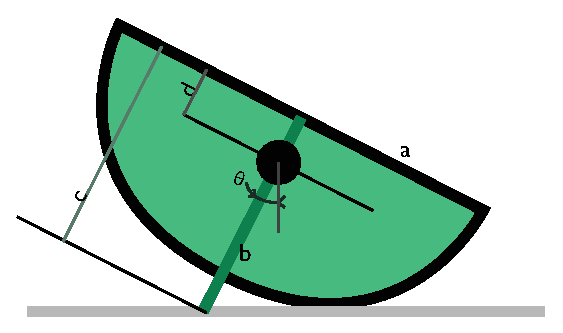
\includegraphics[width=0.5\textwidth]{QS_EnergyAnalysis.eps}
\caption{\label{f:QS_energyGeometry}Geometric Diagram for Tilted Ellipse Energy Analysis}
\end{figure}

Consider Fig. \ref{f:QS_energyGeometry} where $a,b$ are the ellipse's major and minor axes' lengths.
The energy at a given tilt angle $\theta$ will be:

\begin{align}
  E(\theta) =
    \begin{cases}
      mg (c(\theta)-d) \cos(\theta), & \text{if}\ \theta < \frac{\pi}{2} \\
      mg (a \sin(\theta) - d \cos(\theta) ), & \text{if}\ \frac{\pi}{2} \leq \theta < \frac{\pi}{2} + \tan^{-1}(d/a)
    \end{cases}
  \label{eq:QSEnergy}
\end{align}

where $c$ is the minor-axis intercept of the unique tangent line to the semi-ellipse with angle $\theta$ (this tangent defines the ground contact point):

\begin{align}
  c(\theta) \doteq \sqrt{a^2 \tan^2(\theta) + b^2}
\end{align}

\begin{figure}
\centering
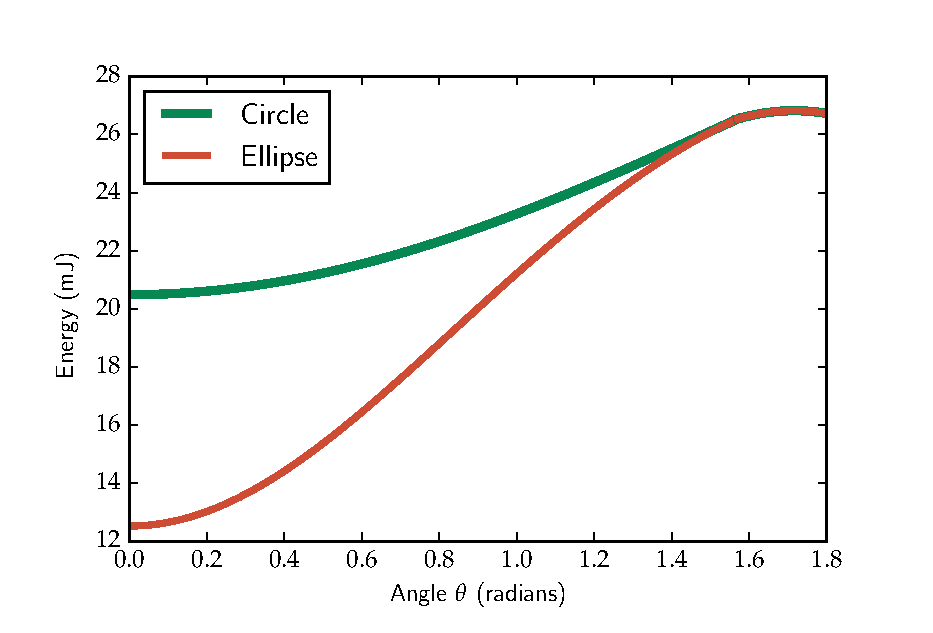
\includegraphics[width=0.5\textwidth]{EnergyLandscape.eps}
\caption{\label{fig:QSEnergy}Energy Landscape over Prone Robot's Angle as described in Eq. \ref{eq:QSEnergy}}
\end{figure}

So that the change in energy required for progression along rotation $\theta$ is:

\begin{align}
  \frac{dE}{d\theta} =
  \begin{cases}
    mg ( (a^2 - b^2) \frac{\sin(\theta)}{\sqrt{a^2 \tan^2(\theta) + b^2}} + d \sin(\theta) ), & \text{if}\ \theta < \frac{\pi}{2} \\
    mg (a \cos(\theta) + d \sin(\theta) ), & \text{if}\ \frac{\pi}{2} \leq \theta < \frac{\pi}{2} + \tan^{-1}(d/a)
  \end{cases}
  \label{eq:QSdEnergy}
\end{align}

This energy differential over position describes how much work must be performed, or how much force is required.
It is plotted in Fig. \ref{fig:QSdEnergy}

\begin{figure}
\centering
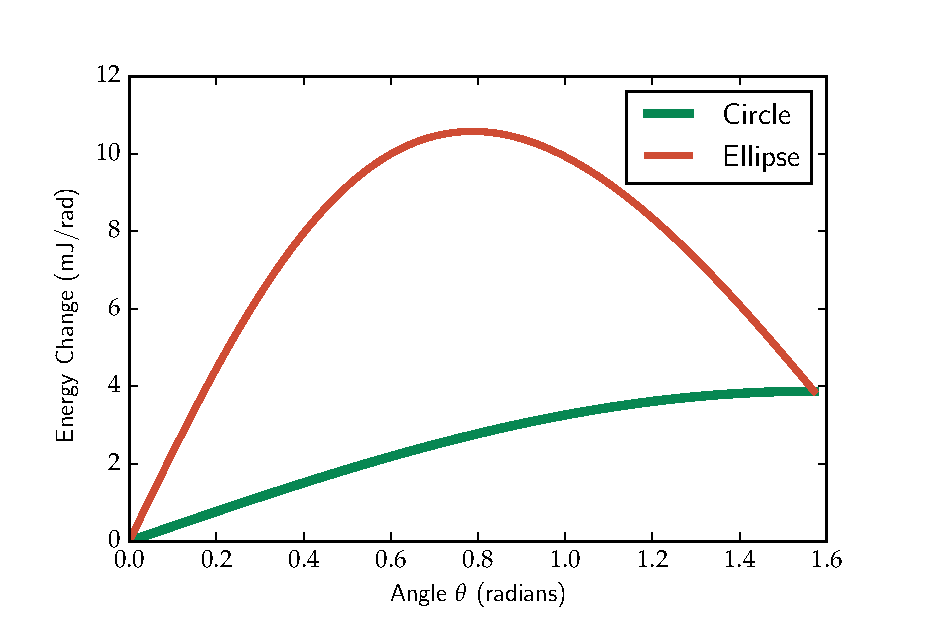
\includegraphics[width=0.5\textwidth]{dEnergyLandscape.eps}
\caption{\label{fig:QSdEnergy}Energy Differential plotted against Angle as described in Eq. \ref{eq:QSdEnergy}}
\end{figure}

Note that the maximum force for pushing a circle in non-decreasing and is maximum at $\theta = \pi/2$ (this will be confirmed again in the below force analysis).
In contrast, the maximum force for pushing an ellipse is much larger and occurs in the middle of the pushing maneuver.
We will see this larger energy requisite manifest as significantly slower pushing maneuvers when operating on ellipses.

\subsubsection{Quasi-static Force Analysis Assumptions}
I have found that the main breaking points for successful quasistatic flipping maneuvers are having the requisite pushing force capacity and sufficient traction between the prone robot's shell and the ground.
To analyze these two variables a simple quasistatic force analysis is sufficient.
Therefore, from the free-body diagram in Fig. \ref{f:QS_FBD} consider the equilibrium equations:

\begin{figure}[ht]
\centering
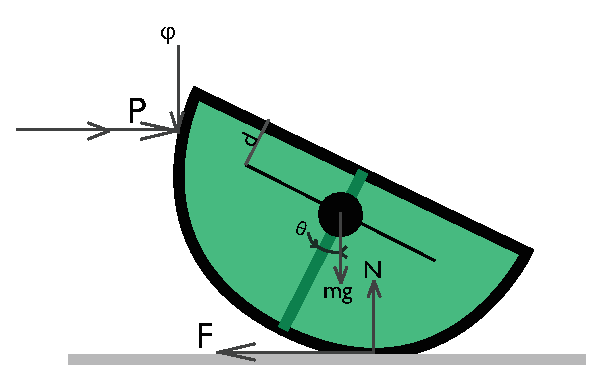
\includegraphics[width=0.5\textwidth]{QS_FreeBodyDiagram2.eps}
\caption{\label{f:QS_FBD}Freebody Diagram for Quasi-static Force and Friction Analysis}
\end{figure}

\begin{align}
  F = P \label{e:QSF_x} \\
  N = mg + \phi \label{e:QSF_y} \\
  P d \cos(\theta) + F(r - d \cos(\theta)) - N d \sin(\theta) - \phi (r - d \sin(\theta)) = 0 \label{e:QSF_o}
\end{align}

We assume the prone robot's shell is sliding along the plow at all times:

\begin{align}
  \phi = \mu P \label{e:QSF_plowFriction}
\end{align}

\subsubsection{Push Force Requisite}
Manipulating Eq. \ref{e:QSF_o} and substituting (in order) Eqs. \ref{e:QSF_x}, \ref{e:QSF_y}, \ref{e:QSF_plowFriction}

\begin{align}
  0 &= P d \cos(\theta) + P(r - d \cos(\theta)) - N d \sin(\theta) - \phi (r - d \sin(\theta))
  \\&= Pr - N d \sin(\theta) - \phi (r - d \sin(\theta))
  \\&= Pr - (mg + \phi) d \sin(\theta) - \phi (r - d \sin(\theta))
  \\&= Pr - mg d \sin(\theta) - \phi r
  \\&= (P - \phi)r - mg d \sin(\theta)
  \\&= (1-\mu) P r - mg d \sin(\theta)
\end{align}

Solving for $P$ yields:

\begin{align}
  P = \frac{mg}{1-\mu} \frac{d}{r} \sin(\theta)
\end{align}

Which means that the pushing robot needs to be able to apply at least the maximum push force required throughout the manipulation:

\begin{align}
  \text{push capacity} \geq P_{max} = \max_\theta \frac{mg}{1-\mu} \frac{d}{r} \sin(\theta) = \frac{mg}{1-\mu} \frac{d}{r}
\end{align}

Note that any friction between the pusher's front surface and the pronated robot's shell increases the required push force.
The requisite push force goes to infinity as $\mu$ approaches unity.
Therefore, we seek to make the friction between the two shells as low as possible.
We will also need a fairly strong pushing robot.

\subsubsection{Friction Requisite}
For this analysis we desire (and assume) that the prone robot is rolling without slip along the ground, thereby constraining the friction force inside the cone described by:

\begin{align}
  F \leq h N \label{e:QSF_groundFriction}
\end{align}

where $h$ is the friction coefficient between the pronated shell and the ground.
Plugging Eq. \ref{e:QSF_x} into the left-hand side of Eq. \ref{e:QSF_groundFriction} and Eq. \ref{e:QSF_y} into the right-hand side (along with Eq. \ref{e:QSF_plowFriction}) yields:

\begin{align}
  P \leq \frac{hmg}{1-h\mu} \label{e:QSF_pushConstraint1} \hspace{5mm} \forall \theta
\end{align}

The tightest bound will be at the $\theta$ when push force is maximized $P_{max}$:

\begin{align}
  P_{max} = \frac{mg}{1-\mu} \frac{d}{r} &\leq \frac{hmg}{1-h\mu} \\
  \frac{1}{1-\mu} \frac{d}{r} &\leq \frac{h}{1-h\mu}
  \label{e:gndFrictionReq}
\end{align}

when we assume the pusher-prone contact is frictionless the requirement on the prone-ground contact reduces to:

\begin{align}
  \frac{d}{r} &\leq h
\end{align}

If the ground friction is insufficient the prone robot will flip up to a specific angle $\theta_{break}$ where the friction constraint is exactly met and then will rotate no further with more pushing.
At the angle $\theta_{break}$ the prone robot will merely slide across the surface when pushed instead of flipping.

\subsection{Experimental Results}
The VelociRoACH robot was equipped with a cylindrical shell and set to walk forwards for 2 seconds after being setup and aimed at another pronated VelociRoACH robot.
The experimental results are summarized in Tbl. \ref{tbl:results}
The flipping maneuver successfully 26 times out of 30 trials. Two of the failures were due to the pushing robot deflecting away from the prone target upon impact.
The other two failures were only due to not running the robot long enough (only 2 seconds).
Both failures will be easily fixed with the addition of a heading controller and flip end-condition check, respectively.
These features were not implemented in this base test for sake of repeatability and to avoid a changing control signal that would confound power estimates.

\begin{table*}[tb]
% increase table row spacing, adjust to taste
\renewcommand{\arraystretch}{1.1}
\caption{Results Table}
\label{tab:Results}
\centering
\begin{tabular}{l l c c}
\hline
Condition Icon\label{tbl:results} & Condition Description & Successes & Avg. Righting Time (ms) \\
\hline
\raisebox{-\totalheight/2}{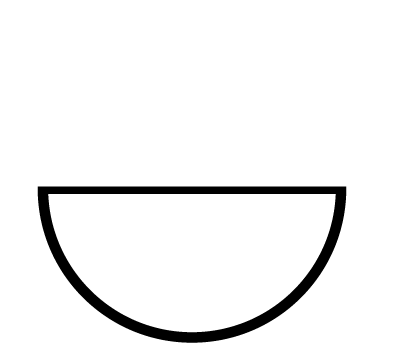
\includegraphics[width=0.05\textwidth]{CircleIcon.png}} & Semi-circular Prism & 26/30 (87\%) & 405.2 ms \\
\raisebox{-\totalheight/2}{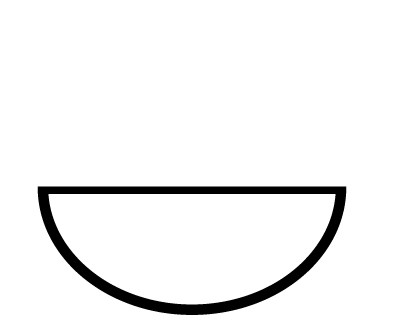
\includegraphics[width=0.05\textwidth]{EllipseIcon.png}} & Semi-elliptical Prism & 15/20 (75\%) & 512.6 ms \\
\hline
\raisebox{-\totalheight/2}{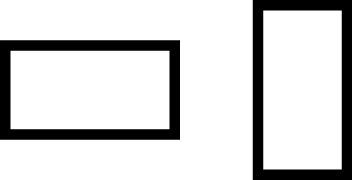
\includegraphics[width=0.05\textwidth]{0Align.png}} & Prism, Straight (0 degree) Alignment & 26/30 (87\%) &  \\
\raisebox{-\totalheight/2}{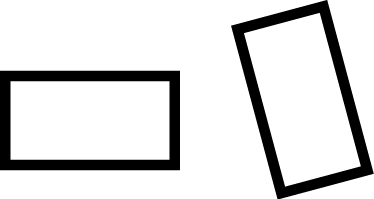
\includegraphics[width=0.05\textwidth]{30Align.png}} & Prism, Scant (30 degree) Alignment & 5/5 (100\%) &  \\
\raisebox{-\totalheight/2}{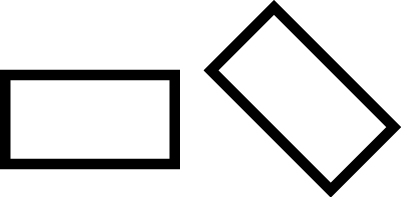
\includegraphics[width=0.05\textwidth]{45Align.png}} & Prism, Scant (45 degree) Alignment & 5/5 (100\%) &  \\
\raisebox{-\totalheight/2}{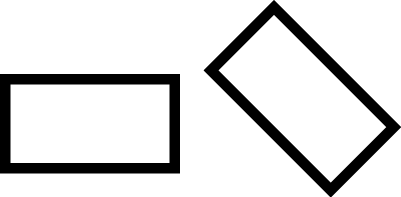
\includegraphics[width=0.05\textwidth]{60Align.png}} & Prism, Scant (60 degree) Alignment & 2/5 (40\%) &  \\
\raisebox{-\totalheight/2}{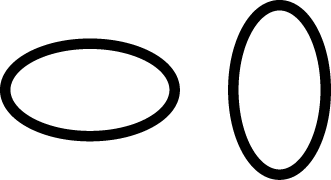
\includegraphics[width=0.05\textwidth]{EllipEllipAlign.png}} & Ellpisoidal, Straight (0 degree) & 0/5 (0\%) & \\
\hline
\raisebox{-\totalheight/2}{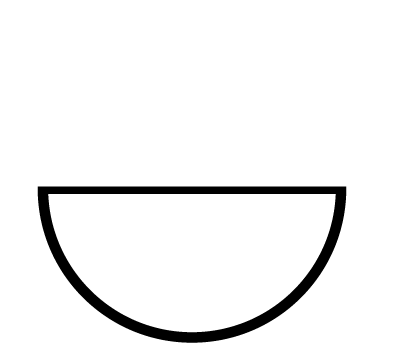
\includegraphics[width=0.05\textwidth]{CircleIcon.png}} & Rubberized Prism & 26/30 (87\%) & 405.2 ms \\
\raisebox{-\totalheight/2}{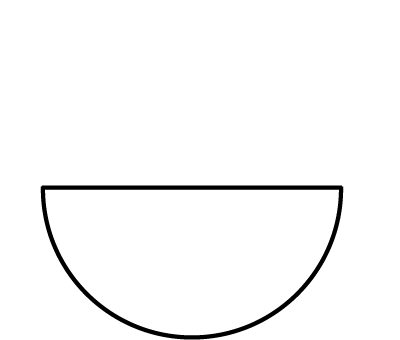
\includegraphics[width=0.05\textwidth]{BareCircleIcon.png}} & Bare Prism & 0/5 (0\%) &  \\
\hline
\end{tabular}
\end{table*}

\subsubsection{Ground Friction Requisite}
As shown in Eq. \ref{e:gndFrictionReq} a minimum shell-ground friction coefficient is necessary to successfully perform a quasi-static flip.
This was tested experimentally by varying the friction coefficient using the added tractive strips made of santoprene rubber.
The successful design condition discussed above (with the 26/30 success rate) used santoprene strips.
When these strips were removed the bare plastic failed to grip the ground and 5/5 flip attempts failed.
This manifested as 3/5 pushes failing due to the prone robot simply skittering away from the pusher, and 2/5 pushes failing after the prone robot twisted (in yaw) away from the push thereby deflecting the pusher off to the side.

\subsubsection{Footrpint Alignment}
In Section \ref{sec:Molds} we chose to narrow designs to prismatic extrustions of 2D shapes, asserting that secondary curvature was actually undesirable.
That assertion was tested experimentally by varying the entry angle of the prismatic robots to assess alignability and was contrasted with the poor experimental alignment performance of ellipsoidal shells.

Robots with the prismatic design (rectangular footprint) will self-align orthogonally when pressed together.
When initialized with alignment (=zero degree offset) the robots stayed align in 28/30 trials.
When initialized with 30 degree, 45 degree, or 60 degree offsets the alignment succeeded in 5/5, 5/5 and 2/5 trials respectively.
Therefore past around a 45 degree offset the self-alignability of the shells drops off.

Then we tested robots pushing with ellipsoidal designs (elliptical footprint).
Even when initialized already aligned the pusher deflected away from the target robot immediately upon contact (successful alignment in 0/10 trials).
This is easily understood from a classical grasping standpoint; the elliptical footprint of the pushing robot contacts the target along its unstable major axis.
This observation also aligns with the design reasoning for why previous shell iterations for the VelociRoACH used ellipsoids: terradynamic streaming.
The goal of ``terradynamic streaming'' is to create exterior hulls for the robot that will slip past obstacles upon collision.
As attested to in this experiment, the ellipsoidal hull is excellent at deflecting away from obstacles.
This selfsame characteristic becomes undesirable when we instead need the robot to transfer force to obstacles it engages.

\section{Dynamic Flip Method}
\subsection{Energetic Analysis}

\begin{align}
E_1 = \frac{1}{2} m_1 v_1^2 \hspace{3mm} = E_2 = \frac{1}{2} I_2 \omega_2^2 \hspace{3mm} = E_3 = m_2 g \sqrt{d^2+r^2}
\end{align}

\section{Discussion}

\section{Future Work}


\section{Conclusion}
To be written second to last.

\section{Acknowledgements}
Many thanks to Carlos Casarez for his indispensable advice on experimental design and analyses as well as general direction on where to take this project.

\bibliographystyle{plain}
\bibliography{manipulation}

\end{document}
